% vim:ft=tex:
%
\documentclass{beamer}

\makeatletter
\def\input@path{{examples}}
% When theme as submodule use the below line instead
% \def\input@path{{usyd-beamer-theme/}}
\makeatother

\usepackage[orientation=portrait,size=a1,scale=1.5,debug]{beamerposter}
\usepackage[utf8]{inputenc}
\usepackage[australian]{babel}
\usepackage{amsmath}
\usepackage{subcaption}
\usepackage{filecontents}

\usepackage[backend=biber,style=phys]{biblatex}
\usepackage{biblatex}
\addbibresource{../examples/references.bib}
\setbeamertemplate{bibliography item}{\insertbiblabel}
\renewcommand*{\bibfont}{\small}

\begin{filecontents*}{references.bib}
@article{Dietz2017,
author = {Dietz, C. and Kretz, T. and Thoma, M. H.},
doi = {10.1103/PhysRevE.96.011301},
journal = {Phys. Rev. E},
number = {1},
pages = {1--5},
title = {{Machine-learning approach for local classification of crystalline structures in multiphase systems}},
volume = {96},
year = {2017}
}
@article{Reinhart2017,
author = {Reinhart, Wesley F. and Long, Andrew W. and Howard, Michael P. and Ferguson, Andrew L. and Panagiotopoulos, Athanassios Z.},
doi = {10.1039/C7SM00957G},
journal = {Soft Matter},
number = {27},
pages = {4733--4745},
publisher = {Royal Society of Chemistry},
title = {{Machine learning for autonomous crystal structure identification}},
url = {http://xlink.rsc.org/?DOI=C7SM00957G},
volume = {13},
year = {2017}
}
@article{scikit-learn,
 title={Scikit-learn: Machine Learning in {P}ython},
 author={Pedregosa, F. and Varoquaux, G. and Gramfort, A. and Michel, V.
         and Thirion, B. and Grisel, O. and Blondel, M. and Prettenhofer, P.
         and Weiss, R. and Dubourg, V. and Vanderplas, J. and Passos, A. and
         Cournapeau, D. and Brucher, M. and Perrot, M. and Duchesnay, E.},
 journal={Journal of Machine Learning Research},
 volume={12},
 pages={2825--2830},
 year={2011}
}
\end{filecontents*}

\addbibresource{references.bib}

\mode<presentation>{\usetheme{usyd-poster}}

\setbeamertemplate{footline}{
  \begin{beamercolorbox}[wd=\paperwidth]{upper separation line foot}
    \rule{0pt}{3pt}
  \end{beamercolorbox}

  \leavevmode%
  \begin{beamercolorbox}[ht=7ex,leftskip=1em,rightskip=1em]{author in head/foot}%
    \hfill
    \small\texttt{mram5995@uni.sydney.edu.au}\hspace{2em}
    \vskip1ex
  \end{beamercolorbox}
  \vskip0pt%
}

\graphicspath{{examples/figures/}{../}}
% Use the below line instead when usyd-beamer-theme is a submodule
% \graphicspath{{figures/}{usyd-beamer-theme/}}

\title{The Detection and Characterisation of \\\vspace{0.3em} Molecular Crystals using Machine Learning}
\author{Malcolm Ramsay}
\institute{School of Chemistry, The University of Sydney}


\begin{document}
\begin{frame}[t]{}
  \begin{columns}[t]

    \begin{column}{0.47\linewidth}

      \begin{block}{Abstract}
        The wide range of crystal structures of a molecular crystal
        can make it difficult to detect and characterise each of them individually.
        Presented, is a general approach to the detection and characterisation
        of local crystalline order using machine learning.
        This approach is able to categorise different crystalline orderings and the liquid phase
        with an accuracy in excess of 95\% over a wide temperature range.
      \end{block}

      \begin{block}{Introduction}
        The molecule we are studying has three distinct crystal structures
        with potential energies all within 2\% of each other.
        \begin{figure}[h]
          \centering
          \begin{subfigure}[t]{0.3\linewidth}
              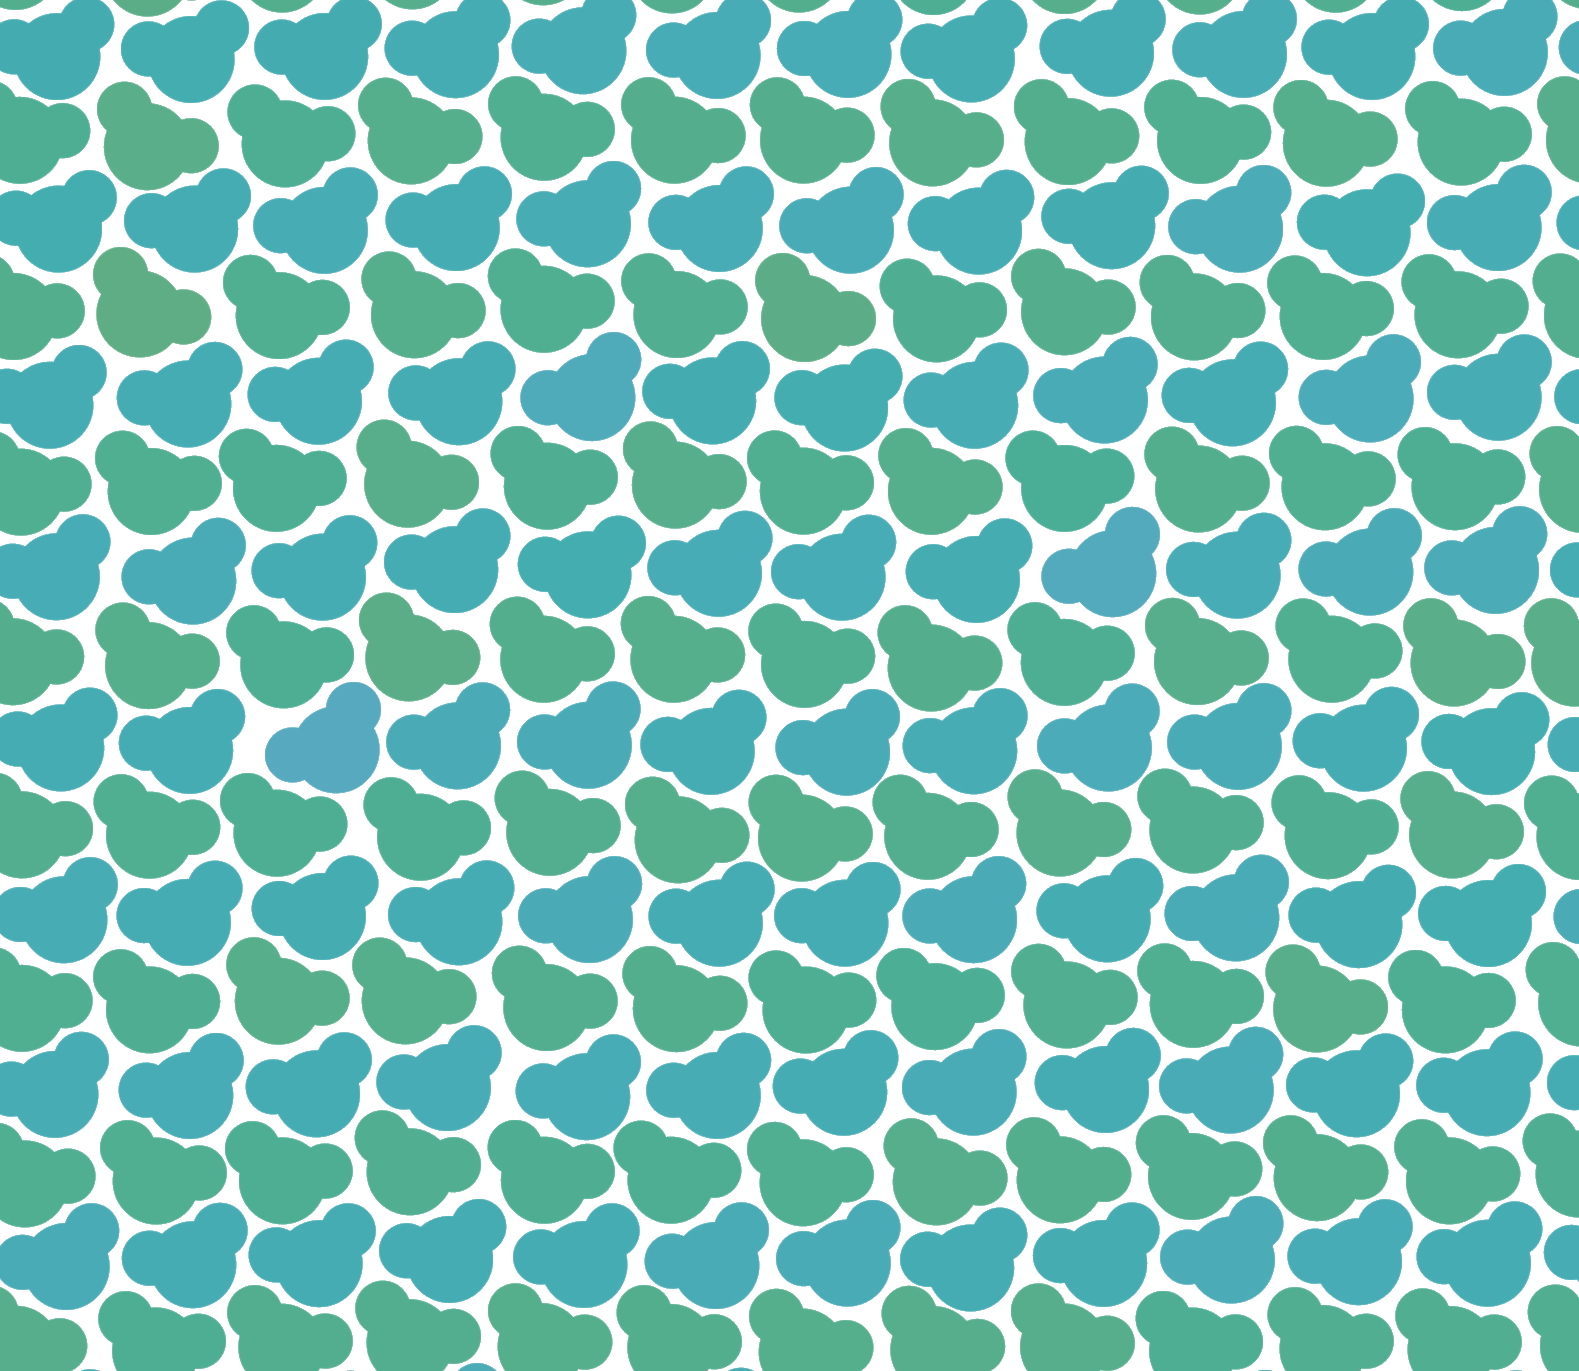
\includegraphics[width=\linewidth]{trimer-crys-pg}
            \caption{pg}
            \label{fig:crystals pg}
          \end{subfigure}
          \begin{subfigure}[t]{0.3\linewidth}
              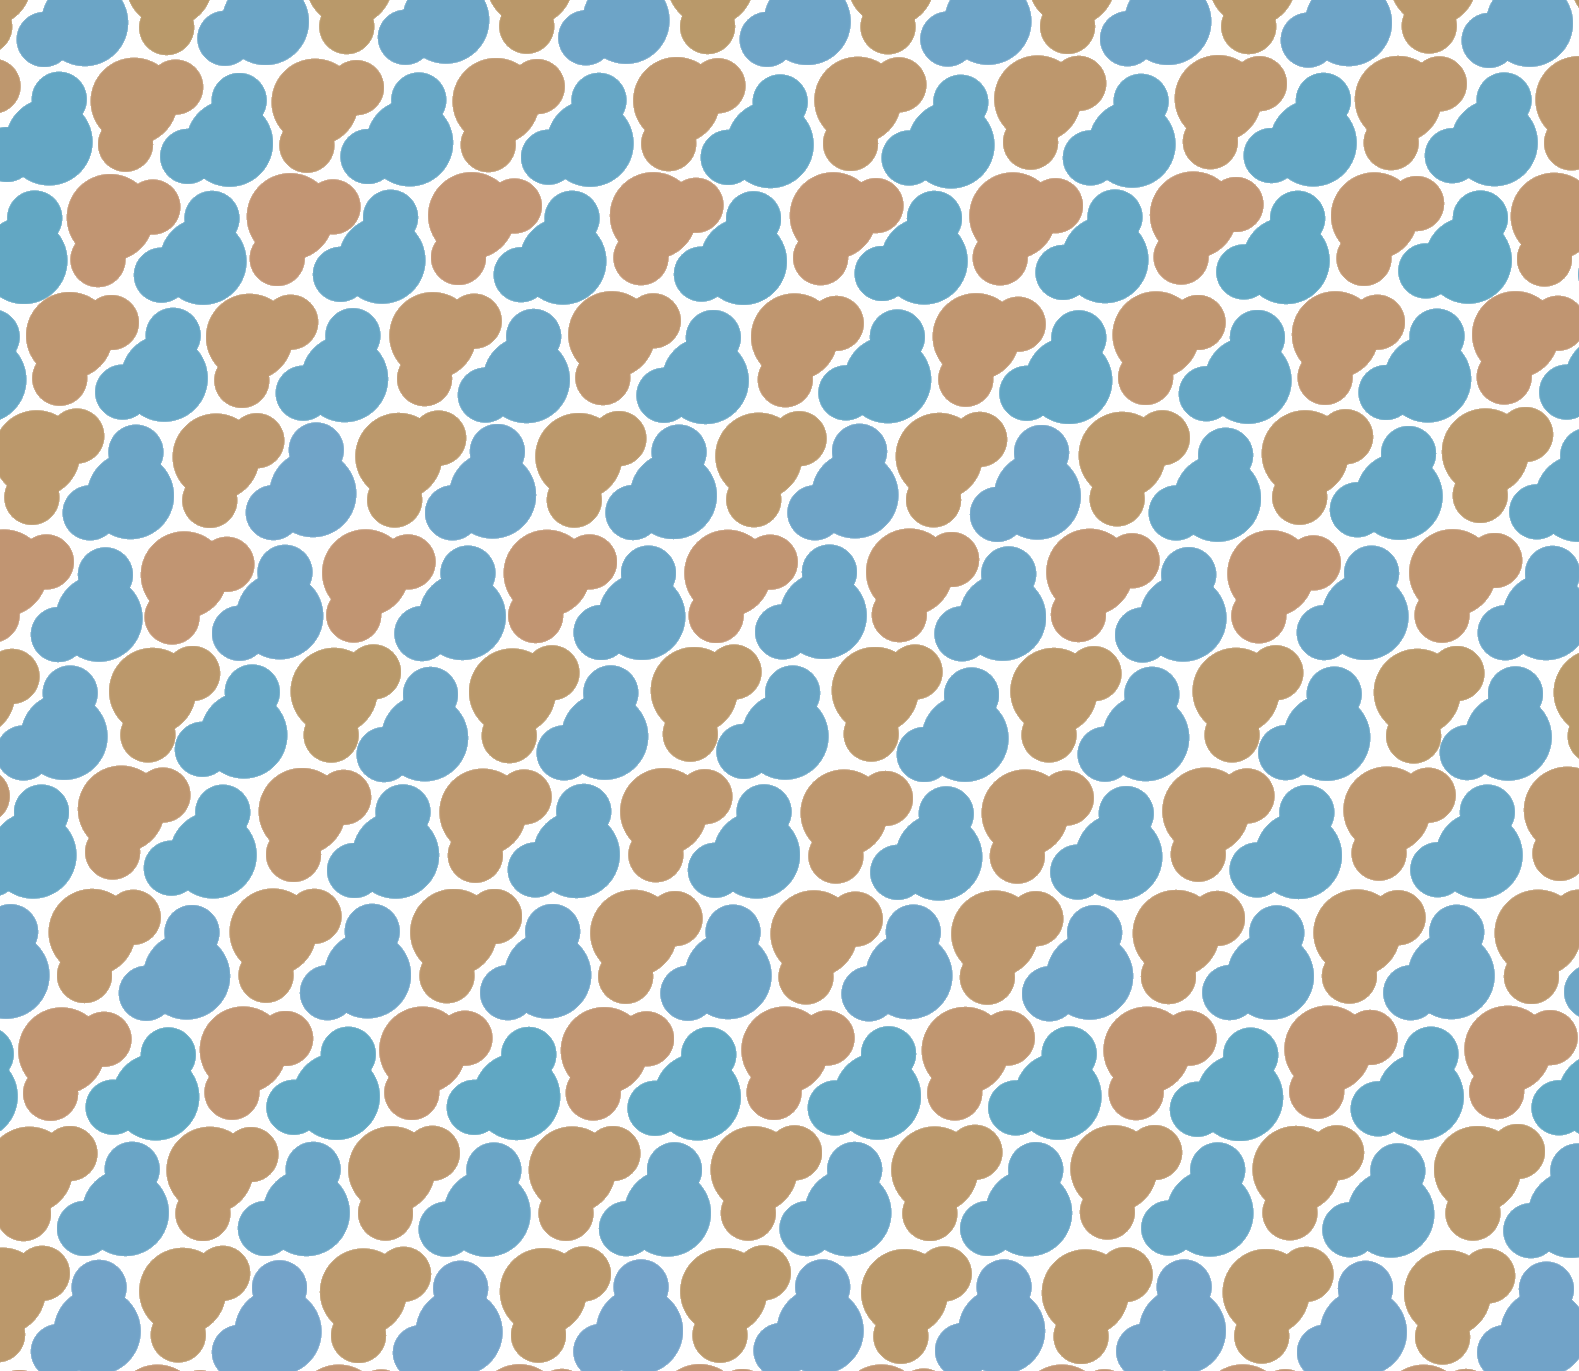
\includegraphics[width=\linewidth]{trimer-crys-p2}
            \caption{p2}
            \label{fig:crystals p2}
          \end{subfigure}
          \begin{subfigure}[t]{0.3\linewidth}
              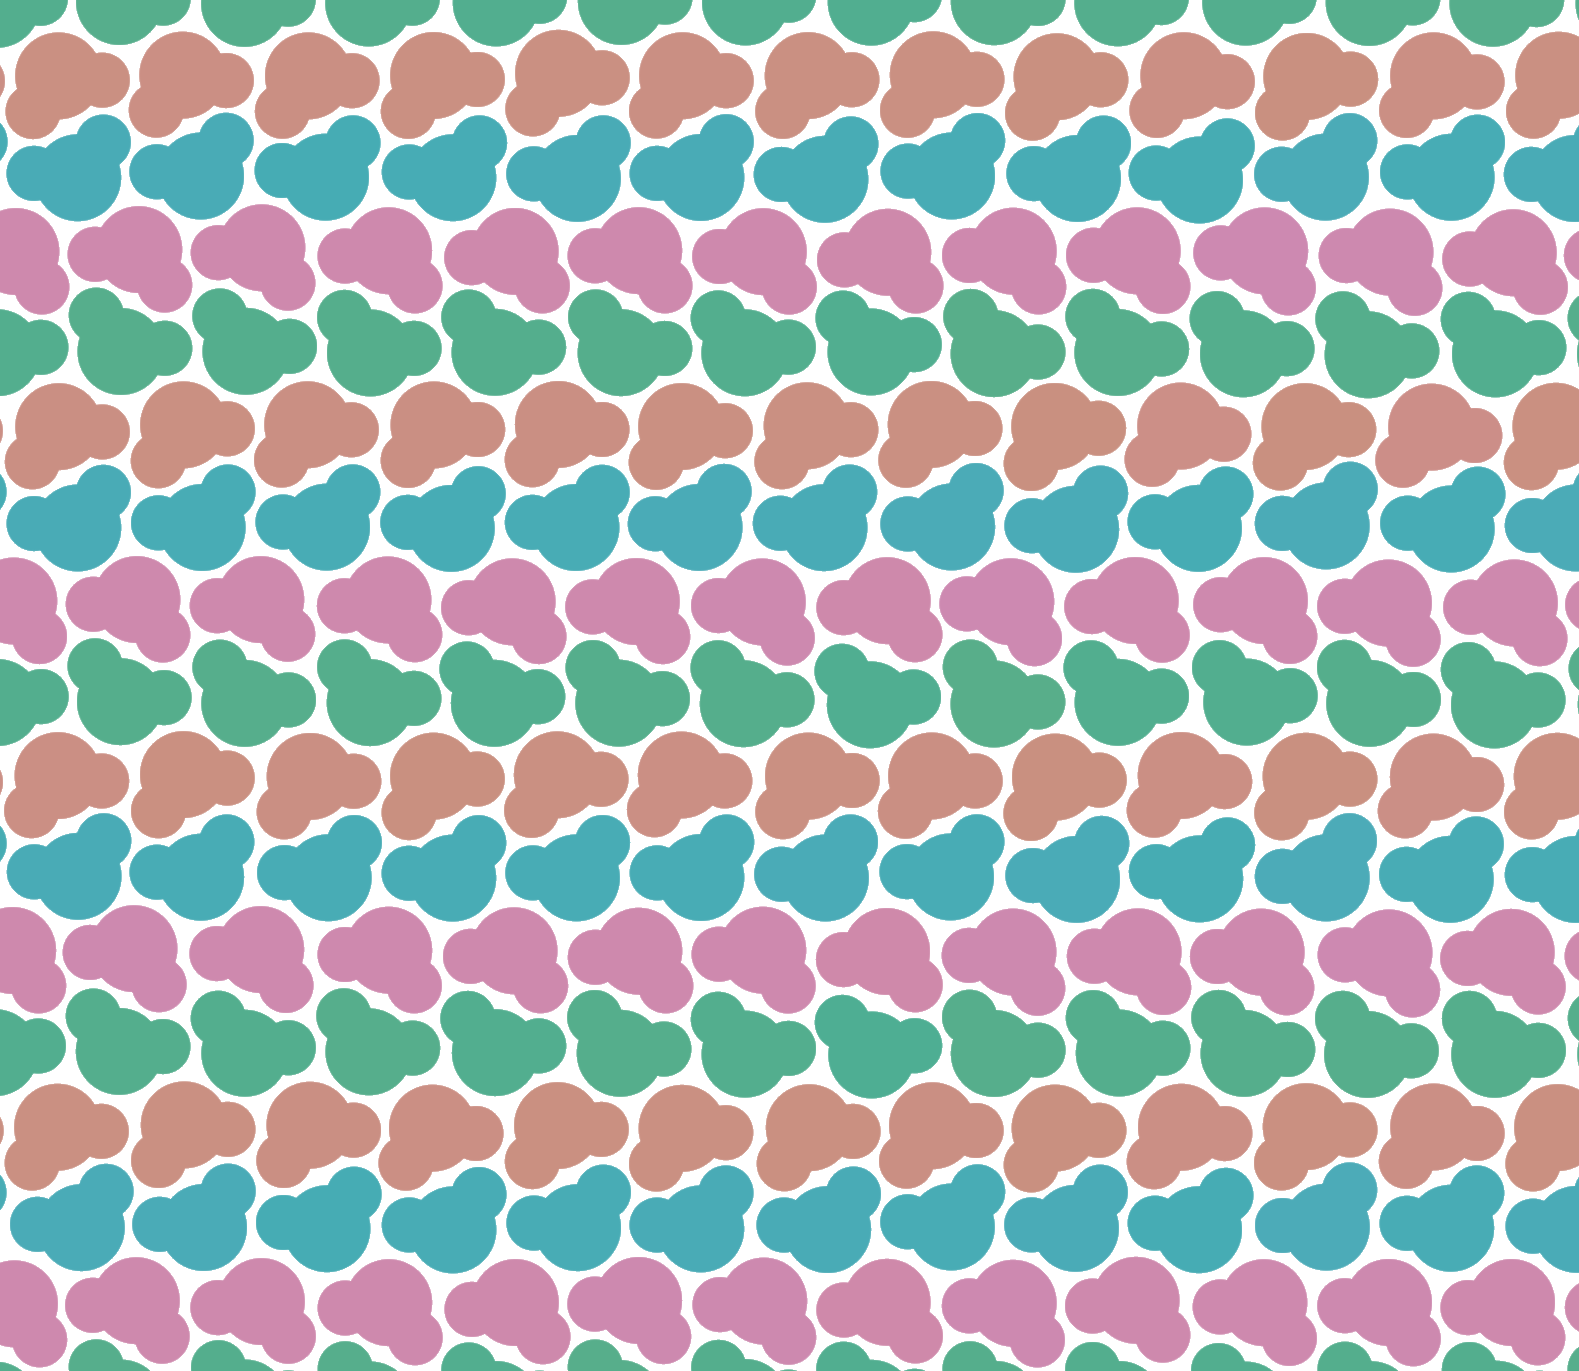
\includegraphics[width=\linewidth]{trimer-crys-p2gg}
            \caption{p2gg}
            \label{fig:crystals p2gg}
          \end{subfigure}
          \caption{The three lowest energy structures of the Trimer molecule.}
          \label{fig:crystals}
        \end{figure}
        A complete understanding of the liquid--solid phase transition requires
        the detection and characterisation of all crystal structures.
        The diversity of structure required metrics and parameters tailored for each structure.

      \end{block}

    \begin{block}{Machine Learning Methodology}

      There has recently been work using machine learning to
      categorize fcc and bcc crystal structures~\autocite{Reinhart2017,Dietz2017} for single atom
      potentials.
      No comparable work was found for molecular crystals.
      The relative orientation of neighbouring molecules was chosen as the feature
      to distinguish crystal structures over a range of temperatures.

      \begin{figure}[h]
        \centering
        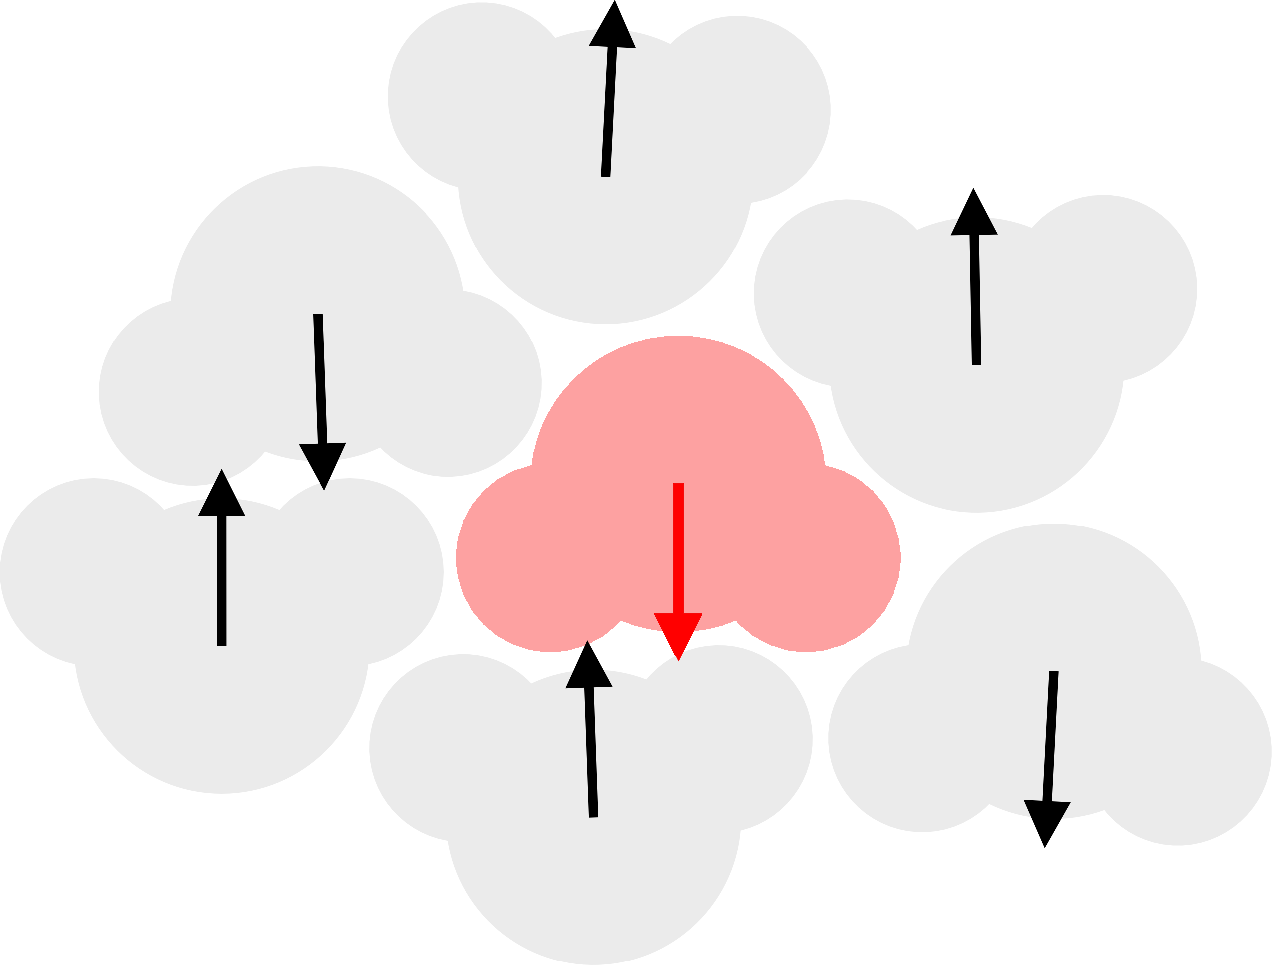
\includegraphics[width=0.6\linewidth]{orientations}
        \caption{The features of a molecule (in red) are the relative orientations of the nearest
        neighbours (grey).}
        \label{fig:orientations}
      \end{figure}

      Machine learning algorithms from the scikit-learn~\autocite{scikit-learn} library
      were used for classification.
      The K-nearest neighbours algorithm gave the best results for this work.

    \end{block}

    \begin{block}{References}
      \printbibliography
    \end{block}

    \end{column}
    \begin{column}{0.47\linewidth}
      \begin{block}{Results}
        A single classification algorithm can be used to monitor melting of all crystals
        with minimal classification errors or noise from thermal fluctuations.

        \begin{figure}[h]
          \centering
          \begin{subfigure}[t]{\linewidth}
            \centering
              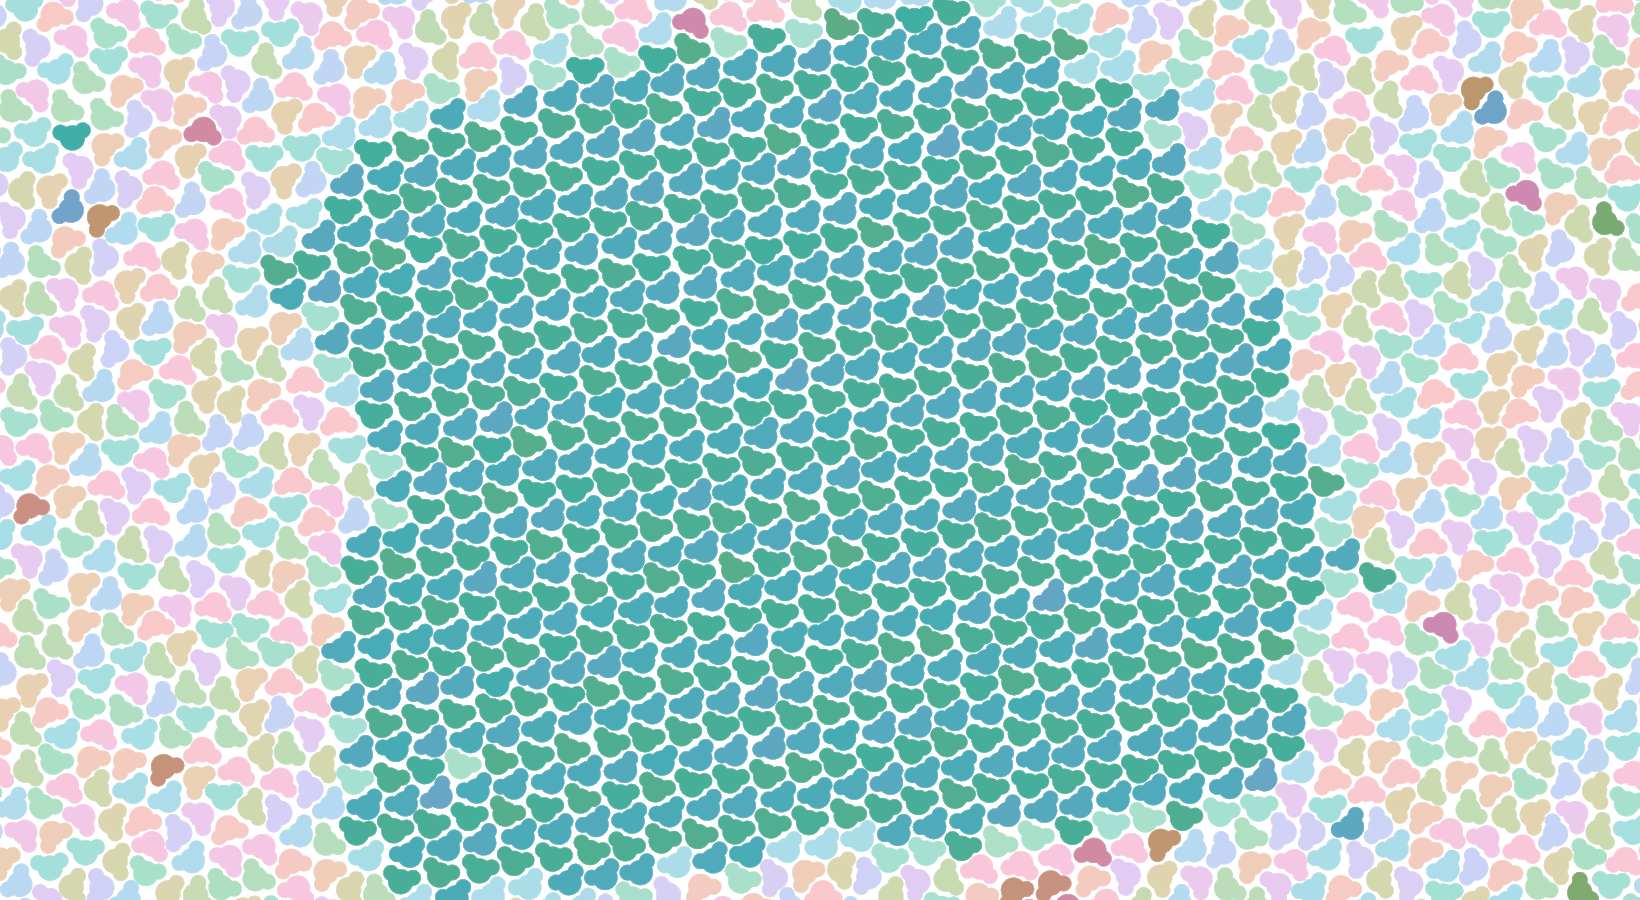
\includegraphics[width=\linewidth]{trimer-cat-pg}
            \caption{pg}
            \label{fig:categorised pg}
          \end{subfigure}
          \begin{subfigure}[t]{\linewidth}
            \centering
              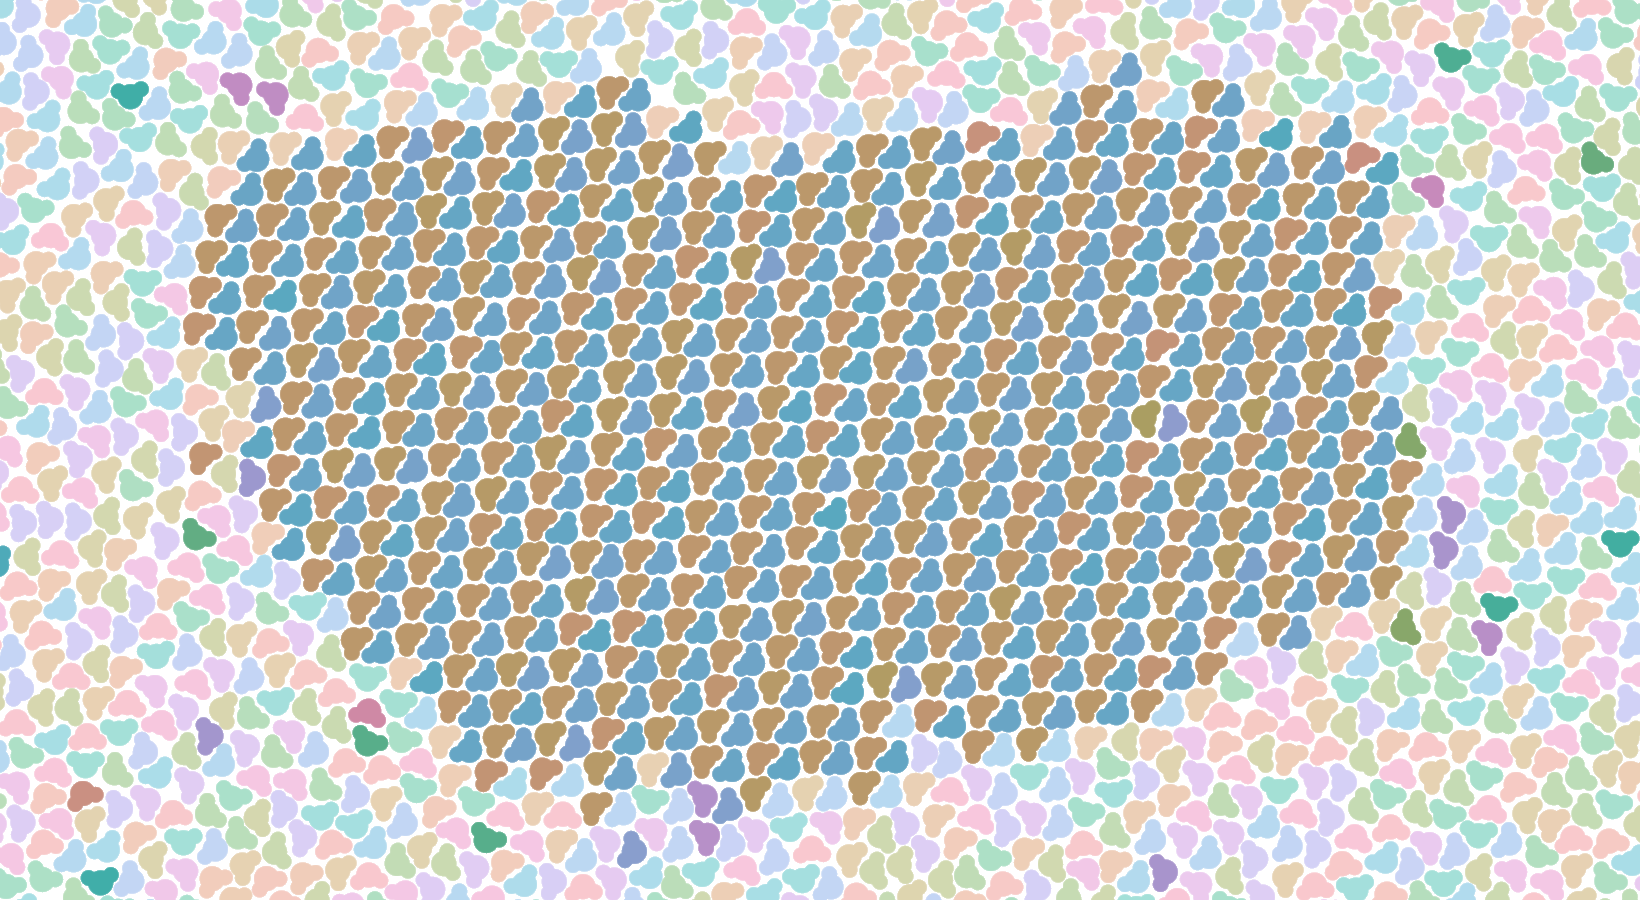
\includegraphics[width=\linewidth]{trimer-cat-p2}
            \caption{p2}
            \label{fig:categorised p2}
          \end{subfigure}
          \begin{subfigure}[t]{\linewidth}
            \centering
              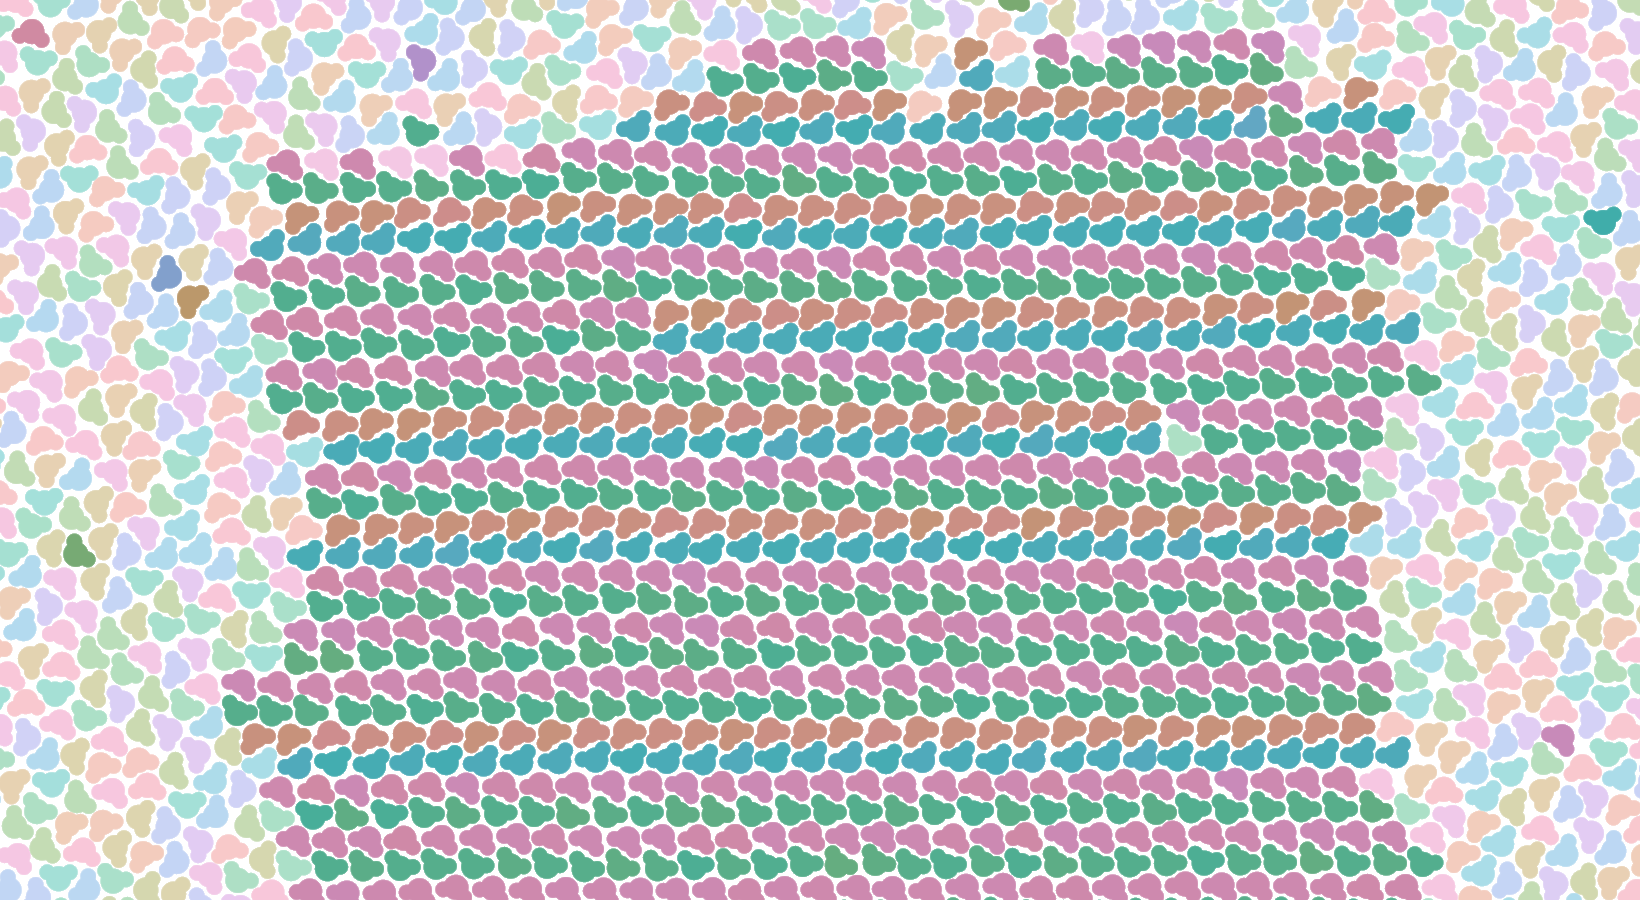
\includegraphics[width=\linewidth]{trimer-cat-p2gg}
            \caption{p2gg}
            \label{fig:categorised p2gg}
          \end{subfigure}
          \caption{Each of the crystal structures characterised using the same
            machine learning algorithm. Regions classified as crystalline are darker
            than those classifies as liquid.}
          \label{fig:categorised}
        \end{figure}

        Note that most of the single molecules classified as crystalline in the liquid
        have a local environment that matches one of the crystals.

      \end{block}

      \begin{block}{Future Work}
        This work could easily be extend to a wide range of crystal structures
        using the relative orientations, a scaled distance, and angle to neighbours.
        This extension requires finding the crystal structures of a number of 3D molecules
        to generate the training data.\\

        Further work would incorporate this functionality into a simple to use open source library
        so that this can become a standard analysis tool for many types of crystals.

      % Hack to align bottoms of columns
      \vspace{0.75em}
      \end{block}

    \end{column}
  \end{columns}
\end{frame}

\end{document}
